\documentclass[tikz,border=5mm]{standalone} 
\usetikzlibrary{positioning, calc}
\usetikzlibrary{angles, quotes}
\begin{document}

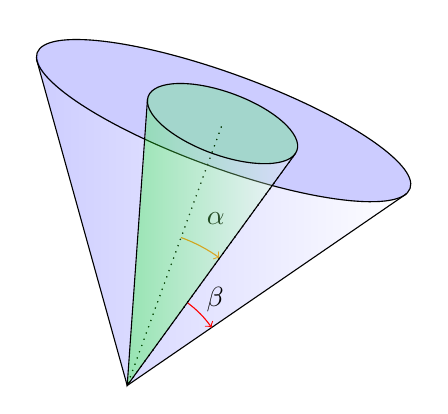
\begin{tikzpicture}
 
  % AK8 variables
  \def\x{2.5}
  \def\y{3.5}
  \def\R{\x+0.02}
  \def\yc{\y+0.08}
  \def\e{0.6}

	 % define point

    % angle  

 
  % AK8 cone
  \begin{scope}[rotate=-20]
  \shade[right color=white,left color=blue,opacity=0.2]
    (-\x,\y) -- (-\x,\yc) arc (180:360:{\R} and \e) -- (\x,\y) -- (0,0) -- cycle;
  \draw[fill=blue,opacity=0.2]
    (0,\yc) circle ({\R} and \e);
  \draw
    (-\x,\y) -- (0,0) -- (\x,\y);
  \draw
    (0,\yc) circle ({\R} and \e);
    
  \coordinate (A)  at (0, 3.5);
  \coordinate (O)  at (0,0);
  \coordinate (B)  at (1,3.5);    
    
  \draw[dotted] (A) -- (O) -- (B);
 % \draw pic[->,"$\alpha_1$",draw=black,angle radius=10,angle eccentricity=1.4]
  %  {angle = B--O--A};    
   \pic["$\alpha$", draw=orange, <-, angle eccentricity=1.2, angle radius=2cm]
    {angle=B--O--A}; 
 
  
  
 \coordinate (AO)  at (1, 3.5);
  \coordinate (OO)  at (0,0);
  \coordinate (BO)  at (2.5,3.5);    
    
  \draw[dotted] (A) -- (O) -- (B);
 % \draw pic[->,"$\alpha_1$",draw=black,angle radius=10,angle eccentricity=1.4]
  %  {angle = B--O--A};    
   \pic["$\beta$", draw=red, <-, angle eccentricity=1.2, angle radius=1.3cm]
    {angle=BO--OO--AO};   
    
    
\end{scope} 

 
 
  % AK4 variables
  \def\x{1.0}
  \def\y{3.5}
  \def\R{\x+0.005}
  \def\yc{\y+0.04}
  \def\e{0.4}
 

 
  % AK4 cone 2
  \begin{scope}[rotate=-20] %rotate -20
    \shade[right color=white,left color=green,opacity=0.3]
      (-\x,\yc) -- (-\x,\yc) arc (180:360:{\R} and \e) -- (\x,\yc) -- (0,0) -- cycle;
    \draw[fill=green,opacity=0.2]
      (0,\yc) circle ({\R} and \e);
    \draw
      (-\x,\y) -- (0,0) -- (\x,\y);
    \draw
      (0,\yc) circle ({\R} and \e);
  \end{scope}
 
\end{tikzpicture}
\end{document}
